\documentclass[aspectratio=169,11pt,hyperref={colorlinks=true}]{beamer}
\usepackage[utf8]{inputenc}
\usepackage[T1]{fontenc}
\usepackage{fontspec}
\usepackage[absolute,overlay]{textpos}
\usepackage{listingsutf8}
\usepackage{listings-golang}
\usepackage{tikz}
\usepackage{color}


\title{Developing a CD pipeline with Knative}
\date[DevOps Meetup]{March 14th 2019, Singapore, Singapore}
\author[Andrea]{
  Andrea Frittoli \\
  Developer Advocate \\
  andrea.frittoli@uk.ibm.com \\
  @blackchip76
}

\usetheme{ibmcloud}

% Code style
\setlststyle

\lstdefinelanguage{koyaml}{
  keywords={github, com, afrittoli, examples, ms, go, helloworld},
  sensitive=false,
  comment=[l]{\#},
  morestring=[b]',
  morestring=[b]"
}

% Automatic section frame
\AtBeginSection{\frame{\sectionpage}}

\begin{document}

\begin{frame}[noframenumbering]
\titlepage{}
\end{frame}

\section{A Bit of History}

% The main points of the talk are:
% - give an introduction to Tekton Pipelines
% - get in some more details with an example
% - talk about Kaniko and source to image with tricky bits
% - reusing tasks, dev vs CI vs CD
% - point of integration with serving and eventing
% - can I use Tekton? Where? security concerns

\begin{lblackrwhiteframe}
  \frametitle{Knative}
  \large
  \begin{beamercolorbox}[wd=0.3\paperwidth]{text}
    \begin{itemize}
      \item Beginning of 2018...
      \item Knative:
      \begin{itemize}
        \item Build
        \item Eventing
        \item Serving
      \end{itemize}
    \end{itemize}
  \end{beamercolorbox}%
  \begin{textblock*}{0.5\paperwidth}(0.5\paperwidth,0.2\paperheight)
    \centering
    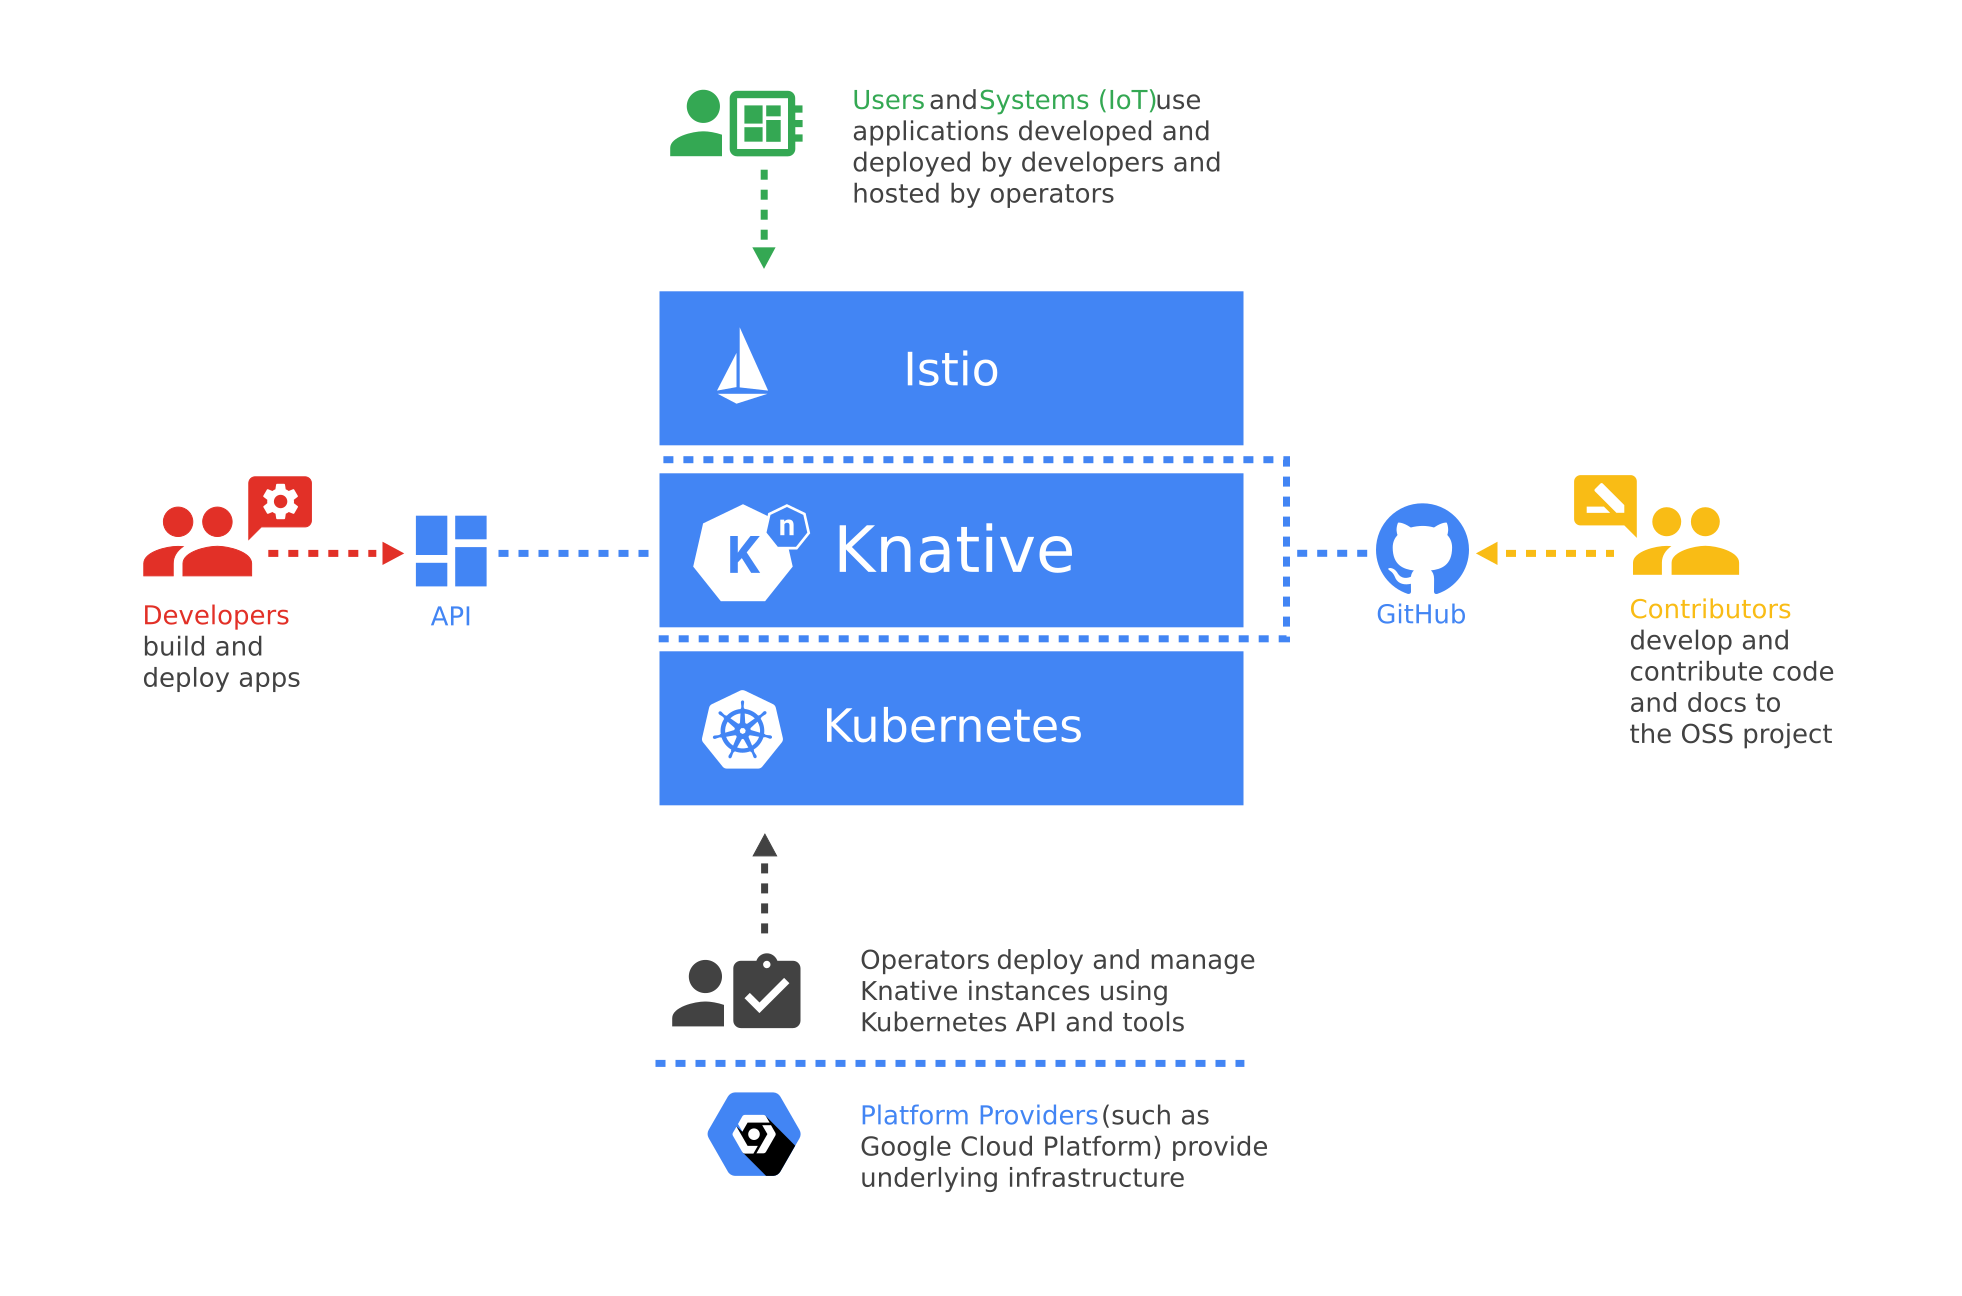
\includegraphics[width=0.45\paperwidth]{img/knative-audience.png}
  \end{textblock*}
\end{grayframe}

\begin{blackframe}
  \frametitle{Knative Pipelines}
  \begin{textblock*}{\paperwidth}(0cm,0.2\paperheight)
    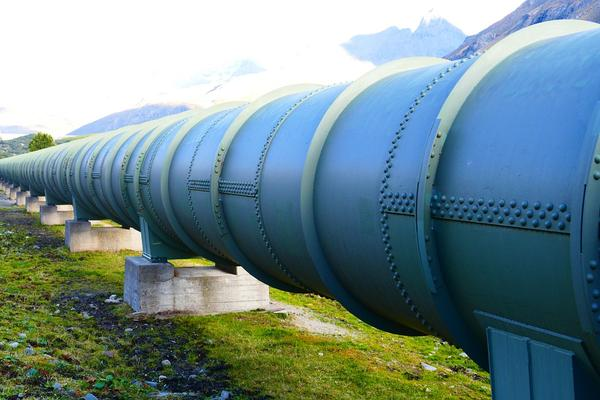
\includegraphics[width=\paperwidth]{img/pipeline_cc0.jpg}
    % https://mediad.publicbroadcasting.net/p/shared/npr/styles/placed_wide/nprshared/201804/605180710.jpg
  \end{textblock*}
  \begin{textblock*}{0.2\paperwidth}(0.83\paperwidth,0.93\paperheight)
    
\includegraphics[width=0.03\paperwidth]{img/cc.png}
    
\includegraphics[width=0.03\paperwidth]{img/zero.png}
  \end{textblock*}
\end{blackframe}

\begin{grayframe}
  \frametitle{Tekton Pipelines}
\end{grayframe}

\begin{grayframe}
  \frametitle{Community}
\end{grayframe}

\section{Tekton Pipelines}

\begin{grayframe}
  \frametitle{Intro}
\end{grayframe}

\begin{grayframe}
  \frametitle{CRDs, Reconcile}
\end{grayframe}

\begin{grayframe}
  \frametitle{Steps, Tasks, Pipelines, Params}
\end{grayframe}

\begin{grayframe}
  \frametitle{*Runs, PipelineResources}
\end{grayframe}

\begin{grayframe}
  \frametitle{Inputs \& Outputs}
\end{grayframe}

\begin{grayframe}
  \frametitle{DAG and ordering}
\end{grayframe}

\begin{grayframe}
  \frametitle{Entrypoint}
  % Entrypoint tools
  % Custom images in Steps
  % PVC vs Object storage
\end{grayframe}

\section{Source to Image to Deploy}

\begin{grayframe}
  \frametitle{The Health Application}
  % components
  % repos
\end{grayframe}

\begin{grayframe}
  \frametitle{IBM Cloud}
  % service accounts
  % the add-on
\end{grayframe}

\begin{grayframe}
  \frametitle{CD Pipeline}
\end{grayframe}

\begin{grayframe}
  \frametitle{Parameters}
  % Environment vs run specific stuff
\end{grayframe}

\begin{grayframe}
  \frametitle{Using Kaniko}
  % Caching layers
  % Base images cache
  % Output image
  % Optimize the docker image
  % Reproducible builds
\end{grayframe}

\begin{grayframe}
  \frametitle{Cluster resource and secrets}
  % Environment vs run specific stuff
\end{grayframe}

\begin{grayframe}
  \frametitle{Service account and namespace}
  % Image Pull and Push
\end{grayframe}

\section{Tekton and Knative}

\begin{grayframe}
  \frametitle{Kservices and Build}
\end{grayframe}

\begin{grayframe}
  \frametitle{Duck Typing and Tekton}
  % Using tasks and pipelines in Kservices
  % Build vs CI
\end{grayframe}

\begin{grayframe}
  \frametitle{Tekton and CI}
  % GitOps Style
  % Challenges
  % Existing integrations
\end{grayframe}

\begin{grayframe}
  \frametitle{Triggering with Eventing}
  % Using tasks and pipelines in Kservices
  % Build vs CI
  % Native triggers: TBD
  % Async pipelines
\end{grayframe}

\section{Conclusions}

\begin{grayframe}
  \frametitle{Roadmap}
\end{grayframe}

\begin{grayframe}
  \frametitle{References}
\end{grayframe}

\section{Q\&A}

\end{document}
